\documentclass[11pt,a4paper]{article}
\usepackage[utf8]{inputenc}
\usepackage[T1]{fontenc}
\usepackage{amsmath,amssymb,amsfonts}
\usepackage{geometry}
\geometry{top=2.3cm, bottom=2.3cm, left=2.3cm, right=2.3cm}
\usepackage{booktabs}
\usepackage{array}
\usepackage{xcolor}
\usepackage{fancyhdr}
\usepackage{hyperref}
\usepackage{enumitem}
\usepackage{tcolorbox}
\usepackage{tabularx}
\usepackage{graphicx}

\renewcommand{\tablename}{Tabla}
\renewcommand{\abstractname}{Resumen}

\definecolor{primary}{RGB}{18, 52, 86}
\definecolor{secondary}{RGB}{41, 128, 185}
\definecolor{darkgray}{RGB}{50, 50, 50}
\definecolor{boxbg}{RGB}{245, 248, 252}
\definecolor{boxframe}{RGB}{41, 128, 185}

\hypersetup{colorlinks=true, linkcolor=secondary, citecolor=secondary, urlcolor=secondary}

\pagestyle{fancy}
\fancyhf{}
\fancyhead[L]{\small \textcolor{darkgray}{Proyecto del Curso - Ambiente, estados y acciones - Team 29}}
\fancyhead[R]{\small \textcolor{darkgray}{\date{\today}}}

\fancyfoot[C]{\thepage}
\renewcommand{\headrulewidth}{0.5pt}

\title{\vspace{-1.5cm}\textbf{\LARGE \textcolor{primary}{Definición de Componentes MDP}}\\[0.3cm]
\Large \textcolor{secondary}{Proyecto del Curso \\
Navegación Autónoma en Entorno Dinámico con Obstáculos}}

\author{\textbf{\tt\small Team 29}\\
{\tt\small \textbf{Silvio Yopasa Romero} \qquad \textbf{Edgar Andrés Pérez Mora}}\\
{\tt\small \{s.yopasa, ea.perezm1\}@uniandes.edu.co}\\
\small Maestría en Inteligencia Artificial (Maia)\\
\small Universidad de los Andes}


\begin{document}
\maketitle
\thispagestyle{fancy}
\hrule \vspace{0.3cm}

\begin{abstract}
Este documento corresponde a la entrega parcial del proyecto del curso de Aprendizaje por Refuerzo. El problema consiste en un agente que debe navegar en una cuadrícula de $8 \times 8$ desde $(0,0)$ hasta $(7,7)$ sin chocar con cinco obstáculos que se mueven de forma aleatoria. \\

En esta entrega se formalizan los componentes del MDP. Primero, el conjunto de estados, donde se especifica el tipo, el rango de valores y los estados terminales de cada variable; asimismo, se propone una representación reducida que permite almacenar los valores en una $Q$-tabla. A continuación, el conjunto de acciones (rotar a la izquierda, rotar a la derecha y avanzar), junto con las reglas que determinan qué acciones aplican en cada estado, incluido lo que pasa cuando el agente está en el borde. Por último, el modelo de recompensas $R(s, a, s')$, donde $s$ es el estado de salida, $a$ la acción ejecutada y $s'$ el estado de llegada.
\end{abstract}

\vspace{0.3cm} \hrule \vspace{0.4cm}

\section{Descripción del ambiente y conjunto de estados ($\mathcal{S}$)}
El problema consiste en un agente de Aprendizaje por Refuerzo (RL) que debe navegar en una cuadrícula de $8 \times 8$ desde $(0,0)$ hasta $(7,7)$ sin chocar con cinco obstáculos que se mueven de forma aleatoria. Cada casilla se identifica con su fila $x$ y su columna $y$, donde $x, y \in \{0, \dots, 7\}$, es decir, $(0,0)$ es la esquina superior izquierda y $(7,7)$ la esquina inferior derecha. En cada paso el agente ejecuta una acción y los obstáculos se mueven a una casilla vecina. El episodio termina cuando el agente llega a la meta (éxito) o cuando choca con un obstáculo (falla).

Para cumplir la \textbf{propiedad de Markov}, el estado debe tener toda la información necesaria para saber qué pasa después de ejecutar una acción, es decir, cuál es el siguiente estado y qué recompensa se recibe. Por eso, el estado en el instante $t$ incluye la posición y la orientación del agente, además de la posición de los cinco obstáculos:
\begin{equation}
    s = \big(x_a, y_a, \theta_a, (x_{o_1}, y_{o_1}), (x_{o_2}, y_{o_2}), (x_{o_3}, y_{o_3}), (x_{o_4}, y_{o_4}), (x_{o_5}, y_{o_5})\big)
\end{equation}

Por ejemplo, si el agente está en la fila 2, columna 3, mirando al Este, y los obstáculos están en $(1,5)$, $(4,4)$, $(6,0)$, $(3,7)$ y $(7,2)$, el estado es $s = \big(2, 3, 1, (1,5), (4,4), (6,0), (3,7), (7,2)\big)$.

\begin{table}[h!]
\centering
\small
\renewcommand{\arraystretch}{1.2}
\caption{Variables, tipos de datos, rangos y descripciones del conjunto de estados $\mathcal{S}$.}
\vspace{0.2cm}
\begin{tabularx}{\textwidth}{@{}>{\raggedright\arraybackslash}p{2.1cm}cc>{\centering\arraybackslash}p{3.0cm}>{\raggedright\arraybackslash}X@{}}
\toprule
\textbf{Componente} & \textbf{Variable} & \textbf{Tipo de dato} & \textbf{Rango de valores} & \textbf{Descripción} \\ \midrule
Posición agente & $x_a$ & Entero & $\{0, \dots, 7\}$ & Índice de fila de la cuadrícula donde se ubica el agente. \\
& $y_a$ & Entero & $\{0, \dots, 7\}$ & Índice de columna donde se ubica el agente. \\ \midrule
Orientación agente & $\theta_a$ & Categórico & $\{0, 1, 2, 3\}$ & Dirección hacia la que mira el agente: $0=\text{Norte}$, $1=\text{Este}$, $2=\text{Sur}$, $3=\text{Oeste}$. \\ \midrule
Obstáculo 1 & $(x_{o_1}, y_{o_1})$ & Par de enteros & $\{0, \dots, 7\}^2$ & Fila y columna del primer obstáculo. \\
Obstáculo 2 & $(x_{o_2}, y_{o_2})$ & Par de enteros & $\{0, \dots, 7\}^2$ & Fila y columna del segundo obstáculo. \\
Obstáculo 3 & $(x_{o_3}, y_{o_3})$ & Par de enteros & $\{0, \dots, 7\}^2$ & Fila y columna del tercer obstáculo. \\
Obstáculo 4 & $(x_{o_4}, y_{o_4})$ & Par de enteros & $\{0, \dots, 7\}^2$ & Fila y columna del cuarto obstáculo. \\
Obstáculo 5 & $(x_{o_5}, y_{o_5})$ & Par de enteros & $\{0, \dots, 7\}^2$ & Fila y columna del quinto obstáculo. \\ \bottomrule
\end{tabularx}
\end{table}

\subsection{Estados terminales}
El conjunto total de estados $\mathcal{S}^+$ incluye los estados terminales, que se dividen en dos casos:
\begin{enumerate}[leftmargin=1.2cm]
    \item \textbf{Éxito ($\mathcal{S}_{\text{meta}}$):} estados donde $(x_a, y_a) = (7, 7)$.
    \item \textbf{Colisión ($\mathcal{S}_{\text{colisión}}$):} estados donde $\exists i \in \{1, \dots, 5\}$ tal que $(x_a, y_a) = (x_{o_i}, y_{o_i})$.
\end{enumerate}

\subsection{Representación reducida para la $Q$-tabla}
El número total de estados es $|\mathcal{S}| = 8 \times 8 \times 4 \times 64^5 \approx 2.75 \times 10^{11}$ ya que el agente puede estar en 8 filas, 8 columnas y mirar en 4 direcciones, y cada uno de los 5 obstáculos puede estar en cualquiera de las 64 casillas. Por eso no es posible guardar una $Q$-tabla con todos ellos. Para reducir este número, el agente no ve la posición exacta de los obstáculos, sino lo que detectan unos sensores locales:
\begin{equation}
    s_{\text{percepción}} = (\Delta x_{\text{meta}}, \Delta y_{\text{meta}}, \theta_a, \text{obs}_{\text{frente}}, \text{obs}_{\text{izq}}, \text{obs}_{\text{der}})
\end{equation}
donde $\Delta x_{\text{meta}} = 7 - x_a$ y $\Delta y_{\text{meta}} = 7 - y_a$ toman valores en $\{0, \dots, 7\}$ y dicen cuántas filas y columnas le faltan al agente para llegar a la meta. $\theta_a$ es la orientación del agente y $\text{obs}_k \in \{0, 1\}$ indica si hay un obstáculo en la casilla de enfrente, a la izquierda o a la derecha, según hacia dónde mira el agente. Con esta representación la tabla queda con $8 \times 8 \times 4 \times 2^3 = 2048$ estados, es decir, $2048 \times 3 = 6144$ entradas, un tamaño que se puede entrenar con $Q$-Learning tabular.

\section{Conjunto de acciones del agente ($\mathcal{A}$)}
En cada paso el agente puede girar en su misma casilla o avanzar una casilla hacia adelante. Las tres acciones posibles son:
\begin{equation}
    \mathcal{A} = \{a_0, a_1, a_2\}
\end{equation}

\subsection{Descripción acciones}
\begin{itemize}[leftmargin=1.2cm]
    \item \textbf{$a_0$ --- Rotar $90^\circ$ a la izquierda:} el agente gira sin moverse de su casilla, es decir, $(x_a, y_a)$ se mantiene y solo cambia la orientación, $\theta'_a = (\theta_a - 1) \pmod 4$. Por ejemplo, si mira al Norte ($0$) pasa a mirar al Oeste ($3$).
    \item \textbf{$a_1$ --- Rotar $90^\circ$ a la derecha:} el agente gira sin moverse en sentido contrario, $\theta'_a = (\theta_a + 1) \pmod 4$. Si mira al Norte ($0$) pasa a mirar al Este ($1$).
    \item \textbf{$a_2$ --- Avanzar:} el agente se mueve una casilla hacia donde está mirando:
    \begin{equation}
        (x'_a, y'_a) = 
        \begin{cases}
            (x_a - 1, y_a) & \text{si } \theta_a = 0 \text{ (Norte)} \\
            (x_a, y_a + 1) & \text{si } \theta_a = 1 \text{ (Este)} \\
            (x_a + 1, y_a) & \text{si } \theta_a = 2 \text{ (Sur)} \\
            (x_a, y_a - 1) & \text{si } \theta_a = 3 \text{ (Oeste)}
        \end{cases}
    \end{equation}

\end{itemize}

En la Figura~\ref{fig:acciones} se muestra cómo funcionan las tres acciones: la orientación del agente se comporta como una brújula de cuatro posiciones ($0$ a $3$) donde girar suma o resta $1$ en módulo $4$, mientras que avanzar lo mueve una casilla en la dirección en la que está mirando.

\begin{figure}[h!]
\centering
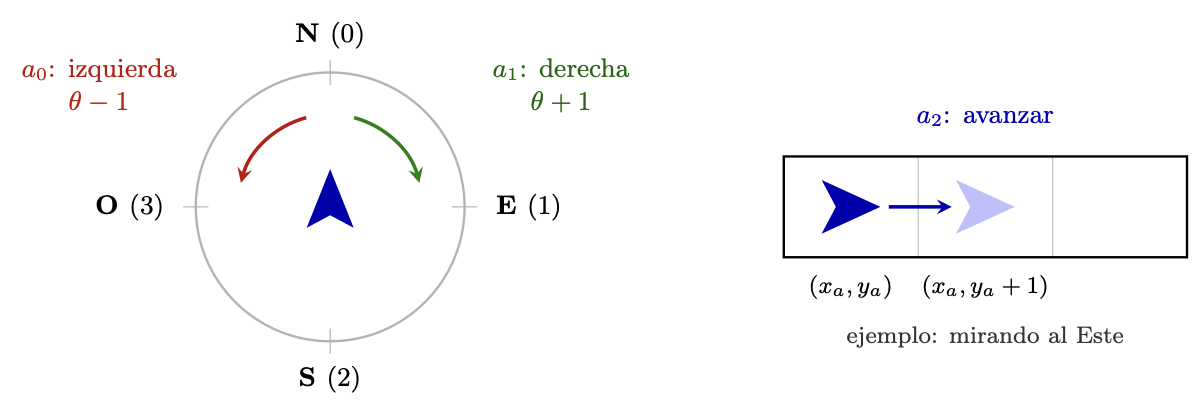
\includegraphics[width=0.75\textwidth]{fig_acciones.png}
\caption{Acciones del agente. }
\label{fig:acciones}
\end{figure}


\subsection{Acciones aplicables en cada estado}
En todos los estados no terminales el agente puede ejecutar las tres acciones, es decir, $\mathcal{A}(s) = \{a_0, a_1, a_2\}$ para todo $s \in \mathcal{S}$. Lo que cambia es el resultado de avanzar cuando el agente está en el borde:
\begin{enumerate}[leftmargin=1.2cm]
    \item \textbf{Rotaciones ($a_0$ y $a_1$):} siempre se pueden ejecutar, porque el agente gira sin cambiar de casilla.
    \item \textbf{Avanzar ($a_2$):}
    \begin{itemize}
        \item \textbf{Si la casilla de llegada está dentro de la cuadrícula}, es decir, $(x'_a, y'_a) \in \{0, \dots, 7\}^2$, el agente se mueve a $(x'_a, y'_a)$.
        \item \textbf{Si la casilla de llegada queda por fuera de la cuadrícula}, el agente choca con la pared y se queda en la misma casilla, $(x'_a, y'_a) = (x_a, y_a)$, además de recibir una penalización. Por ejemplo, si está en $(0, 3)$ mirando al Norte y avanza, sigue en $(0, 3)$.
    \end{itemize}
\end{enumerate}

\section{Modelo de Recompensas y Evaluación}
Según la hipótesis de recompensa de Sutton y Barto, el objetivo del agente se puede expresar como maximizar la suma de recompensas que recibe a lo largo del episodio. Por eso, cada transición se evalúa con un número que indica qué tan buena fue, y ese número depende de la tripla $(s, a, s')$.
\subsection{Mecanismo asignación de recompensas }
La recompensa de cada transición se define según cuatro casos posibles:
\begin{equation}
    R(s, a, s') = 
    \begin{cases}
        \mathbf{+100.0} & \text{si } (x'_a, y'_a) = (7, 7) \quad \text{[Llegada a la meta]} \\
        \mathbf{-100.0} & \text{si } \exists i \in \{1,\dots,5\} : (x'_a, y'_a) = (x'_{o_i}, y'_{o_i}) \quad \text{[Colisión con obstáculo]} \\
        \mathbf{-5.0}   & \text{si } a = a_2 \text{ y } (x'_a, y'_a) = (x_a, y_a) \text{ por chocar con la pared} \\
        \mathbf{-1.0}   & \text{en cualquier otro paso a una casilla libre y no terminal}
    \end{cases}
\end{equation}

\begin{figure}[h!]
\centering
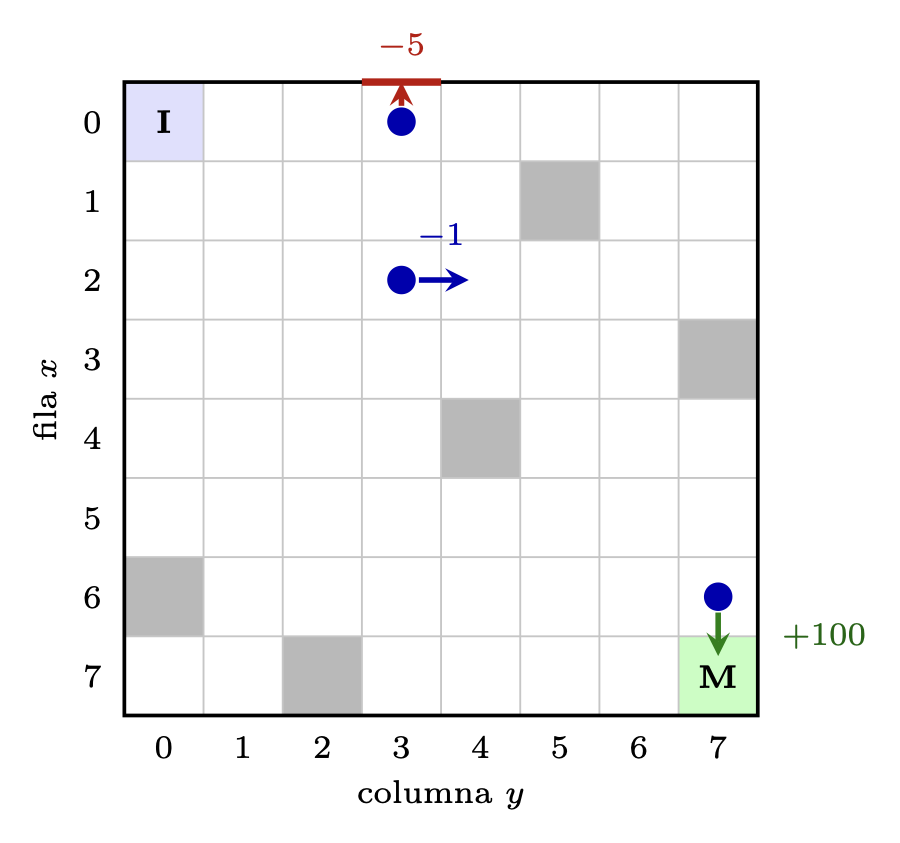
\includegraphics[width=0.55\textwidth]{fig_recompensas.png}
\caption{Ejemplos de recompensas para tres triplas $(s, a_2, s')$.}
\label{fig:ejemplo_recompensas}
\end{figure}

En la Figura~\ref{fig:ejemplo_recompensas}  se muestran tres ejemplos de cómo se aplican estas reglas cuando el agente ejecuta la acción de avanzar ($a_2$) desde distintas casillas. Si está en $(6, 7)$ mirando al Sur, llega a la meta en $(7, 7)$ y recibe $+100$. En cambio, si está en $(2, 3)$ mirando al Este, pasa a la casilla libre $(2, 4)$ y recibe el costo de paso de $-1$, que sirve para que el agente busque el camino más corto. Por último, si está en $(0, 3)$ mirando al Norte, intenta salir de la cuadrícula, choca con la pared, se queda en $(0, 3)$ y recibe $-5$.

\begin{table}[h!]
    \centering
    \small
    \renewcommand{\arraystretch}{1.2}
    \caption{Modelo de recompensas triplas $(s, a, s')$.}
    \label{tab:recompensas}
    \vspace{0.2cm}
    \begin{tabularx}{\textwidth}{@{}>{\raggedright\arraybackslash}p{2.5cm} >{\raggedright\arraybackslash}p{4.5cm} >{\centering\arraybackslash}p{2.2cm} >{\raggedright\arraybackslash}X@{}}
    \toprule
    \textbf{Evento} & \textbf{Condición sobre $(s, a, s')$} & \textbf{Recompensa} & \textbf{Propósito} \\ \midrule
    \textbf{Llegada a la meta} & $(x_a, y_a) \neq (7, 7) \land (x'_a, y'_a) = (7, 7)$ & \textbf{$+100.0$} & Recompensa positiva cuando el agente llega a la meta, que es el objetivo principal del episodio. \\ \midrule
    \textbf{Colisión con obstáculo} & $\exists i : (x'_a, y'_a) = (x'_{o_i}, y'_{o_i})$ & \textbf{$-100.0$} & Penalización alta cuando el agente choca con un obstáculo, para que aprenda a esquivarlos. \\ \midrule
    \textbf{Choque con la pared} & $a = a_2 \land (x'_a, y'_a) = (x_a, y_a)$ en el borde & \textbf{$-5.0$} & Penaliza cuando el agente intenta avanzar hacia afuera de la cuadrícula y se queda en la misma casilla. \\ \midrule
    \textbf{Paso libre} & $s'$ no es terminal y no hay choque & \textbf{$-1.0$} & Costo por cada paso para evitar que el agente se quede dando vueltas y busque el camino más corto. \\ \bottomrule
    \end{tabularx}
\end{table}

\section{Dinámica de transición del ambiente ($P$)}
En cada paso, el cambio de estado $s$ al siguiente estado $s'$ depende de dos movimientos que ocurren al mismo tiempo:
\begin{itemize}[leftmargin=1.2cm]
    \item \textbf{Movimiento del agente:} es determinístico, ya que al elegir una acción $a$ se sabe exactamente en qué casilla y con qué orientación queda el agente, según las reglas de la Sección 2.
    \item \textbf{Movimiento de los obstáculos:} es aleatorio. Cada obstáculo $i \in \{1, \dots, 5\}$ se mueve al azar a una de sus casillas vecinas libres, todas con la misma probabilidad:
    \begin{equation}
        \Pr\big((x'_{o_i}, y'_{o_i}) \mid (x_{o_i}, y_{o_i})\big) = \frac{1}{|\mathcal{N}_{\text{libres}}(x_{o_i}, y_{o_i})|}
    \end{equation}
    donde $|\mathcal{N}_{\text{libres}}(x_{o_i}, y_{o_i})|$ es la cantidad de casillas vecinas libres que tiene ese obstáculo.
\end{itemize}
En la Figura~\ref{fig:transicion} se muestra un paso completo en el tablero de $8 \times 8$: el agente en $(2,3)$ avanza a $(2,4)$ sin azar ($p = 1$), mientras que cada uno de los cinco obstáculos ($o_1$ a $o_5$) reparte su probabilidad en partes iguales entre las casillas vecinas libres que tiene ($1/4$ en el interior, $1/3$ en el borde o junto a otro obstáculo, y $1/2$ en una esquina o cuando tiene dos lados bloqueados).

\begin{figure}[h!]
\centering
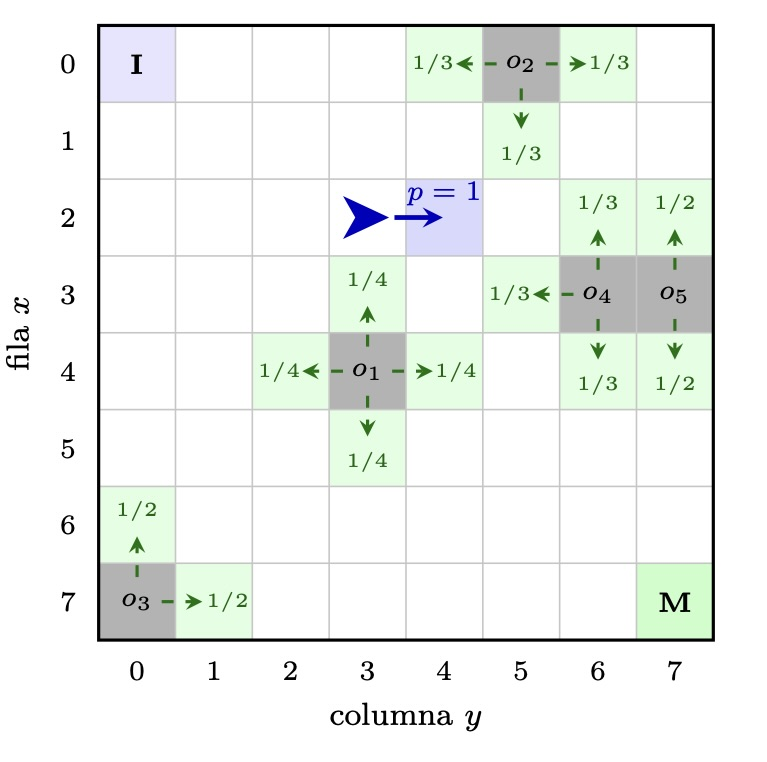
\includegraphics[width=0.52\textwidth]{fig_transicion.png}
\caption{Dinámica de transición en ambiente sobre el tablero.}
\label{fig:transicion}
\end{figure}

\end{document}